\documentclass{article}
%% Useful packages
\usepackage[utf8]{inputenc}
\usepackage[a4paper,left=1.75cm,right=1.75cm,top=2.5cm,bottom=2.5cm]{geometry}
\usepackage{crop,graphicx,amsmath,array,color,amssymb,fancyhdr,lineno}
\usepackage{flushend,stfloats,amsthm,chngpage,times,,lipsum,lastpage} 
\usepackage{calc,listings,color,wrapfig,tabularx,longtable,enumitem}
\usepackage[style=numeric-comp,backend=biber,sorting=none]{biblatex}
\lstset{ language=bash }
\newcommand{\omissis}{[\ldots]\hspace{3pt}}
\usepackage[bottom]{footmisc}
\addbibresource{Refs.bib}
\usepackage{float}
\usepackage{enumitem}
\usepackage[table]{xcolor}
\usepackage{xcolor}
\usepackage{hyperref}
\hypersetup{
    colorlinks=true,
    linkcolor=black,     
    urlcolor=blue,
    citecolor=purple
    }
\urlstyle{same}
%%%%%%%%%%%%   Header and Footer  %%%%%%%%%%%%%
\pagestyle{fancy}
\fancypagestyle{plain}{%
  \renewcommand{\headrulewidth}{0pt}%
  \fancyhf{}%
}

\title{%
  Project 3 \\
  \large Fuzz testing of an image manipulation software using \textit{AFL}}
\author{Marco Ruvolo}

\begin{document}
\begin{titlepage}

\newcommand{\HRule}{\rule{\linewidth}{0.5mm}} % Defines a new command for the horizontal lines, change thickness here

%----------------------------------------------------------------------------------------
%	LOGO SECTION
%----------------------------------------------------------------------------------------
\center

\includegraphics[width=10cm]{Title/logo Sapienza (rgb).png}\\[1cm] % Include a department/university logo - this will require the graphicx package
 
%----------------------------------------------------------------------------------------

\center % Center everything on the page

%----------------------------------------------------------------------------------------
%	HEADING SECTIONS
%----------------------------------------------------------------------------------------

\textsc{\LARGE Sapienza University of Rome}\\[1.5cm] % Name of your university/college
\textsc{\Large Master's degree in Cybersecurity}\\[0.5cm] % Major heading such as course name
\textsc{\large Department of Computer Science}\\[0.5cm] % Minor heading such as course title

%----------------------------------------------------------------------------------------
%	TITLE SECTION
%----------------------------------------------------------------------------------------
\makeatletter
\HRule \\[0.4cm]
{ \huge \bfseries \@title}\\[0.4cm] % Title of your document
\HRule \\[1.5cm]
 
%----------------------------------------------------------------------------------------
%	AUTHOR SECTION
%----------------------------------------------------------------------------------------

\begin{minipage}{0.4\textwidth}
\begin{flushleft} \large
\emph{Author:}\\
\@author % Your name
\\[1.2em]
\emph{Matricola number:}\\
1883257 \\[1.2em]
\end{flushleft}
\end{minipage}
~
\begin{minipage}{0.4\textwidth}
\begin{flushright} \large
\emph{Professor:} \\
Daniele Friolo  \\[1.2em] % Supervisor's Name
\emph{Course:} \\
Security in Software Applications
\end{flushright}
\end{minipage}\\[2cm]
\makeatother

% If you don't want a supervisor, uncomment the two lines below and remove the section above
%\Large \emph{Author:}\\
%John \textsc{Smith}\\[3cm] % Your name

%----------------------------------------------------------------------------------------
%	DATE SECTION
%----------------------------------------------------------------------------------------
\vfill % Fill the rest of the page with whitespace
{\large \today}\\[2cm] % Date, change the \today to a set date if you want to be precise



\end{titlepage}

\sffamily

\fancyhf{}
\fancyhead[L]{}
\fancyhead[R]{}
\fancyfoot[R]{ \bf\thepage\ \rm }%

\newpage
\tableofcontents
\listoffigures
\listoftables
\pagebreak

\section{Introduction to testing and fuzzing}
\label{sec:intro}

\subsection{Testing}
Software testing is a fundamental part of any \textit{SDLC} (Software Development Life Cycle) and it consists in examining the artifacts and the behavior of the software (under test) by validation and verification.

There exist different levels and techniques of software testing:
\begin{itemize}[itemsep=1pt]
    \item \textsc{scenario testing} - to ensure that requirements are complete and consistent (e.g., analysing abuse and misuse cases);
    \item \textsc{specification testing} - to prove the specfication is complete and correct (e.g., through a formal proof or symbolic execution);
    \item \textsc{in-line testing} - to verify invariants, rules and that the internal state of the software is allowed by the security policies, expected and self-consistent (e.g., using assertions);
    \item \textsc{unit testing} - to locally test software units, modules and components;
    \item \textsc{human interaction testing}: to ensure the \textit{UI} (User Interface) and error messages are properly usable (e.g., analysing \textit{UI} abuse cases);
    \item \textsc{integration testing} - to test logically integrated software units, modules and components as a combined entity;
    \item \textsc{final testing} - to run test cases against the entire project (e.g., injecting random input);
    \item \textsc{acceptance testing} - to determine whether the requirements of the specification and customer contract are met.
\end{itemize}

In general, testing does one of the following:
\begin{itemize}[itemsep=1pt]
    \item it looks at correct or wanted behaviour for sensible input or some input on borderline conditions (i.e., normal testing);
    \item it looks for wrong or unwanted behaviour for \textit{bizarre} input (i.e., security testing).
\end{itemize}
Since a normal use of the system is more likely to reveal functional problems than security problems, users complain about the former ones while malicious users never complain about the latter ones.

\subsection{Fuzz testing}
Fuzzing, also known as fuzz testing, was proposed by Barton Miller\parencite{Miller} at the University of Wisconsin in 1988.
Basically, fuzz testing consists of running the software application to test with random input, identifying the eventual crashes and correlating the input that caused the crashes: it is an effective technique for automated security testing.
The basic idea is to see whether the application tested crashes with semi-automatically generate random input.

Initially, fuzzing generated very long input (to make it likely that buffer overruns cross segmentation boundaries) to see whether the system crashes with segmentation fault. Other typical input that can be used for fuzzing could be:
\begin{itemize}[itemsep=1pt]
    \item long strings;
    \item empty string;
    \item maximum and minimum integer values;
    \item zero and negative integer values;
    \item null values;
    \item newline, \textit{EOF} (End Of File) and format string characters;
    \item semicolons, slashes, backslashes, single quotes, double quotes;
    \item application specific keywords (e.g., \textit{DROP TABLE} for \textit{SQL}).
\end{itemize}

Nowadays, there have been developed several kind of fuzzing tools which use \textit{smarter} techniques to generate input:
\begin{itemize}[itemsep=1pt]
    \item (blackbox) mutation-based fuzzers, in which random mutations are applied to existing valid input;
    \item (blackbox) generation-based (also known as grammar-based fuzzers), in which input is generated from some knowledge of format or protocol (e.g., grammar defining legal input, data format specifications);
    \item (greybox) evolutionary fuzzers, that perform mutations using a genetic algorithm;
    \item whitebox fuzzers, that analyze the code to determine interesting input (e.g., using symbolic execution).
\end{itemize}

Tha main weaknesses of generation-based and mutation-based fuzzers are that a huge amount of work is needed to set up the fuzzers and the chance that random changes in input hit interesting cases is small, respectively.

Thus, an evolutionary approach overcomes these downsides: the basic idea is to learn interesting mutations based on measuring code coverage (i.e., if a mutation of the input triggers a new execution path through the code, then it is an interesting mutation and it is kept else it is discarded).

One of these evolutionary tools will be described in the following subsection.

\subsection{A fuzz testing tool: \textit{AFL}}
\textit{AFL}\parencite{AFL} (American Fuzzy Lop) is a security-oriented fuzzer that employs a novel type of compile-time instrumentation and genetic algorithms to automatically discover clean, interesting test cases that trigger new internal states in the targeted binary.

In particular, the mutation strategies used include the following\parencite{AFL_status}.
\begin{itemize}[itemsep=1pt]
    \item \textit{bitflip L/S} - deterministic bit flips: \textit{L} bits are toggled at any given time, walking the input file with \textit{S}-bit increment (the current \textit{L/S} variants are: 1/1, 2/1, 4/1, 8/8, 16/8, 32/8).
    \item \textit{arith L/8} - deterministic arithmetics: the fuzzer tries to subtract or add small integers to 8-, 16-, and 32-bit values (the stepover is always 8 bits).
    \item \textit{interest L/8} - deterministic value overwrite: the fuzzer has a list of known \textit{interesting} 8-, 16-, and 32-bit values to try (the stepover is 8 bits).
    \item \textit{extras} - deterministic injection of dictionary terms: this can be shown as "user" or "auto", depending on whether the fuzzer is using a user-supplied dictionary or an auto-created one.
    \item \textit{havoc} - a sort-of-fixed-length cycle with stacked random tweaks: the operations attempted during this stage include bit flips, overwrites with random and \textit{interesting} integers, block deletion, block duplication, plus assorted dictionary-related operations (if a dictionary is supplied in the first place).
    \item \textit{splice} - a last-resort strategy that kicks in after the first full queue cycle with no new paths: it is equivalent to \textit{havoc}, except that it first splices together two random inputs from the queue at some arbitrarily selected midpoint.
\end{itemize}

Please check the technical "whitepaper" for \textit{afl-fuzz}\parencite{AFL_tech}, to explore in-depth technical details and benchmarks.

\subsection{Project repository}
The project track carried out, the results collected, the plots within this report and this latter itself, are collected in an online \textit{GitHub}\parencite{github} repository.

For further information please visit the following link: \href{https://github.com/mrcruv/afl_fuzzing}{https://github.com/mrcruv/afl\_fuzzing}.
\pagebreak

\section{A case study: \textit{ImageMagick}}
\label{sec:afl}
\textit{ImageMagick}\parencite{IM} is a free and open-source software suite for displaying, converting, and editing raster image and vector image files that can read and write over two hundred image file formats, and can support a wide range of image manipulation operations.

\textit{ImageMagick} is written in \textit{C}, it is available for a wide range of operating systems, including \textit{Linux}, \textit{macOS}, and \textit{Windows} and it can be used as a standalone application, or as a library that can be integrated into other software programs.

The testing phases of the \textit{ImageMagick-6.5.4.-10}\parencite{IM6} (legacy) release, using \textit{AFL}, are reported in the following subsections.

\subsection{Program instrumentation for use with \textit{AFL}}
Since the source code of the major \textit{ImageMagick} releases are available on the \textit{ImageMagick}'s official site (for further information please visit the following link: \href{https://imagemagick.org/archive/releases/}{https://imagemagick.org/archive/releases/}), the target program is compiled as follows\parencite{AFL_guide}\parencite{AFL_readme}.
\begin{lstlisting}
$ CC=<path_to_afl_gcc> CXX=<path_to_afl_g++> ./configure --disable-shared
$ AFL_HARDEN=1 AFL_INST_RATIO=100 make clean all
$ make install
\end{lstlisting}
To link the executable that reads data from a file and passes it to the \textit{ImageMagick} library against this latter itself (or to make sure that the correct .so file is loaded at runtime), a static build is performed (i.e., \textit{--disable-shared} flag).
Moreover, \textit{AFL\_HARDEN} is set to 1 (i.e., \textit{AFL\_HARDEN=1}) in order to enable code hardening options that make it easier to detect simple memory bugs\parencite{AFL_readme}\parencite{AFL_env} and \textit{AFL\_INST\_RATIO}\parencite{AFL_env} is set to 100 (i.e., \textit{AFL\_INST\_RATIO=100}) for allowing the generation of instrumentation for 100\% of branches.


\subsection{Initial test cases choice}
The fuzzer requires an initial test cases corpus that contains a representative sample of the input data normally expected by the targeted application in order to operate correctly.
The two basic rules to follow are the following\parencite{AFL_readme}:
\begin{enumerate}[itemsep=1pt]
    \item keep the files small, for a matter of performance (under 1 kB is ideal, although not strictly necessary);
    \item use multiple tes cases only if they are functionally different from each other.
\end{enumerate}

The \textit{afl-cmin} utility is used to identify a subset of functionally distinct test cases that exercise different code paths in the target binaries, as follows.
\begin{lstlisting}
$ afl-cmin -i <testcase_dir> -o <new_testcase_dir> -- <tested_program> [...]
\end{lstlisting}

Indeed, a subset of \textit{PNG} images is drawn out from the \textit{png} directory inside the \textit{afl\_testcases} directory\parencite{AFL_testcases}, to arrange an initial test cases corpus.
More precisely, the \textit{afl-cmin} utility is used on the images located on the \textit{afl\_testcases/png/full/images} path.

Please note that the \textit{afl-tmin} utility may be used to minimize each test case in a test cases corpus, as follows.
\begin{lstlisting}
$ afl-tmin -i <testcase> -o <new_testcase> -- <tested_program> [...]
\end{lstlisting}

\subsection{Fuzzing binaries}
The fuzzing process itself is carried out by the \textit{afl-fuzz} utility, which requires a read-only directory with initial test cases, a separate directory to store its findings and a path to the binary to test.

For target binaries that accept input directly from \textit{stdin}, the usual syntax is as follows\parencite{AFL_guide}\parencite{AFL_readme}.
\begin{lstlisting}
$ afl-fuzz -i <testcase_dir> -o <findings_dir> -- <tested_program> [...]
\end{lstlisting}

For programs that take input from a file, marking the location in the target's command line where the input file name should be placed is needed, using "@@", as follows\parencite{AFL_guide}\parencite{AFL_readme}.
\begin{lstlisting}
$  afl-fuzz -i <testcase_dir> -o <findings_dir> -- <tested_program> @@ [...]
\end{lstlisting}
Please note that the flags \textit{-t} and \textit{-m} may be used to override the default timeout and memory limit for the executed process, if needed.

Since the \textit{C} function tested in this case study takes input from files, the latter syntax is used.

\subsection{Parallelize fuzzing}
In order to fully exploit the hardware (since a multi-core system is used), fuzzing parallelization is necessary: every instance of \textit{afl-fuzz} takes up roughly one core\parencite{AFL_readme}.

For parallelizing a single job across multiple cores on a local system, \textit{N} instances of \textit{afl-fuzz} should be ran, as follows\parencite{AFL_par}.
\begin{lstlisting}
$ afl-fuzz -i <testcase_dir> -o <sync_dir> -M fuzzer01 -- <tested_program> [...]
$ afl-fuzz -i <testcase_dir> -o <sync_dir> -S fuzzer02 -- <tested_program> [...]
$ ...
$ afl-fuzz -i <testcase_dir> -o <sync_dir> -S fuzzer0N -- <tested_program> [...]
\end{lstlisting}
The first fuzzer is the \textit{master} instance, the following ones are \textit{secondary} instances.
The output directory is shared by all the instances of \textit{afl-fuzz} and each fuzzer will keep its state in a separate subdirectory.
The difference between the \textit{-M} and \textit{-S} modes is that the \textit{master} instance will still perform deterministic checks, while the \textit{secondary} instances will proceed straight to random tweaks.
Please note that running multiple \textit{master} instances is usually wasteful, although there is an
experimental support for parallelizing the deterministic checks.

Monitoring the progress of the jobs from the command line is possible, using the \textit{afl-whatsup} tool as follows\parencite{AFL_par}. 
\begin{lstlisting}
$ afl-whatsup <sync_dir>
\end{lstlisting}

Furthermore, graphs for any active fuzzing task can be generated using the \textit{afl-plot} utility, as follows\parencite{AFL_readme}.
\begin{lstlisting}
$ afl-plot <state_dir> <output_dir>
\end{lstlisting}

\subsection{Output interpretation}
The fuzzing process will create and update, in real time, three subdirectories (actually, for each fuzzer instance) within the output directory\parencite{AFL_readme}:
\begin{itemize}[itemsep=1.5pt]
    \item queue: test cases for every distinctive execution path, plus all the starting files given by the user;
    \item crashes: \textit{unique} test cases that cause the tested program to receive a fatal signal (e.g., \textit{SIGSEGV}, \textit{SIGILL}, \textit{SIGABRT}), grouped by the received signal itself;
    \item hangs: \textit{unique} test cases that cause the tested program to time out.
\end{itemize}
Any existing output directory can be also used to resume aborted jobs, as follows\parencite{AFL_readme}.
\begin{lstlisting}
$ afl-fuzz -i- -o <findings_dir> -- <tested_program> [...]
\end{lstlisting}

Please note that crashes and hangs are considered \textit{unique} if the associated execution paths involve any state transition not seen in previously-recorded faults.
\pagebreak

\section{Result analysis}
\label{sec:res}

\textit{Convert} is the function tested in the case study analysed in this report: three fuzzer instances are ran (one \textit{master} instance and two \textit{secondary} instances) and the minimised test cases corpus previously described (i.e., the minimised \textit{afl\_testcases/png/full/convert\_min} corpus) is used.

The results carried out from the fuzzing process are quantitatively collected in table \ref{tab:convert_results} and discussed below.

%Number of files used o Number of mutations generated
%– Time needed
%– Number of flaws found
%– Are the flaws found known CVEs?
\begin{table}[H]
    \centering
    \begin{tabular}{|c|c|c|c|c|}
        \hline
        \cellcolor{lightgray}\textsc{Fuzzer instance} & \cellcolor{lightgray}\textsc{\# Files used} & \cellcolor{lightgray}\textsc{\# Mutations generated} & \cellcolor{lightgray}\textsc{Time needed} & \cellcolor{lightgray}\textsc{\# Crashes found} \\
        \hline
        \textit{convert\_master} (M) & 6 & 6438 & $\simeq$ 3days & 715 (36 \textit{unique})\\
        \hline
        \textit{convert\_slave1} (S) & 6 & 7151 & $\simeq$ 3days & 6753 (396 \textit{unique}) \\
        \hline
        \textit{convert\_slave2} (S) & 6 & 7114 & $\simeq$ 3days & 6590 (386 \textit{unique}) \\
        \hline
        TOTAL & 6 & 20703 & $\simeq$ 3days & 14058 (818 \textit{unique}) \\
        \hline
    \end{tabular}
    \caption{overall results}
    \label{tab:convert_results}
\end{table}

Here follow some graphs representing the execution trend of the three fuzzer instances ran.

\begin{figure}[H]
    \centering
    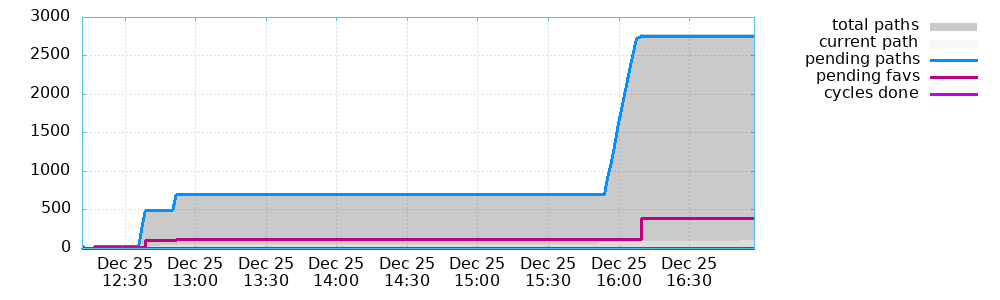
\includegraphics[width=0.5\textwidth]{Resources/convert_master/high_freq.png}\hfill
    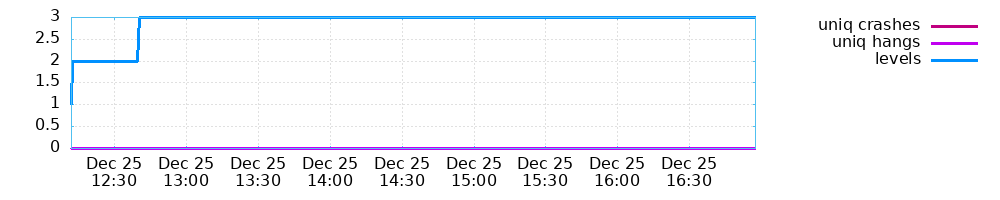
\includegraphics[width=0.5\textwidth]{Resources/convert_master/low_freq.png}
    \caption{execution trend of the \textit{master} instance \textit{convert\_master} for the first 4 hours of processing}
    \label{fig:convert_master}
\end{figure}

\begin{figure}[H]
    \centering
    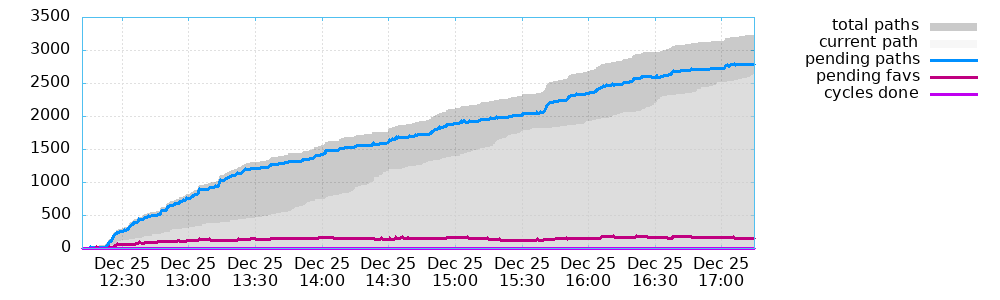
\includegraphics[width=0.5\textwidth]{Resources/convert_slave1/high_freq.png}\hfill
    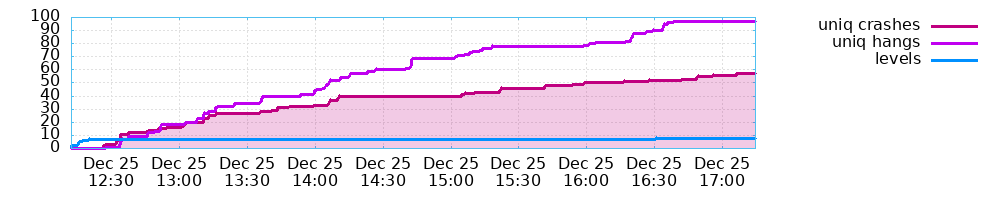
\includegraphics[width=0.5\textwidth]{Resources/convert_slave1/low_freq.png}
    \caption{execution trend of the first \textit{secondary} instance \textit{convert\_slave1} for the first 4$\frac{1}{2}$ hours of processing}
    \label{fig:convert_slave1}
\end{figure}

\begin{figure}[H]
    \centering
    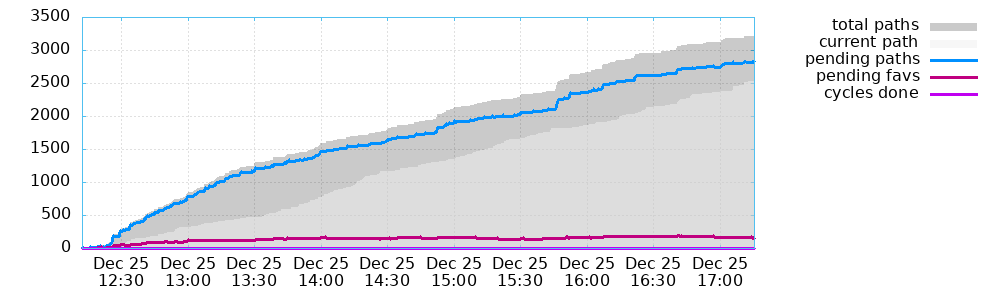
\includegraphics[width=0.5\textwidth]{Resources/convert_slave2/high_freq.png}\hfill
    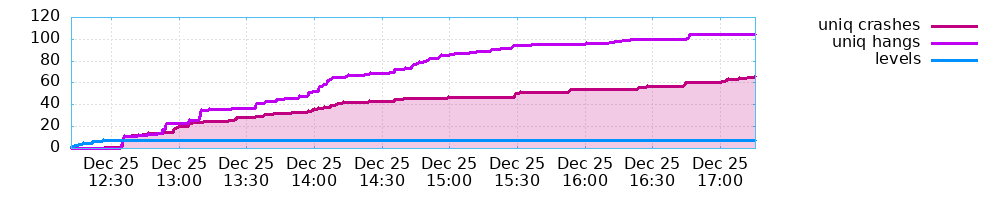
\includegraphics[width=0.5\textwidth]{Resources/convert_slave2/low_freq.png}
    \caption{execution trend of the second \textit{secondary} instance \textit{convert\_slave2} for the first 4$\frac{1}{2}$ hours of processing}
    \label{fig:convert_slave2}
\end{figure}

\subsection{Dynamic result analysis}
The crashes identified by the fuzzing process are grouped by the received signal, for instance\parencite{signals}:
\begin{description}[itemsep=0.5pt]
    \item[sig$\cdot$11]: \textit{SIGSEV} (i.e., invalid memory access - segmentation fault);
    \item[sig$\cdot$07]: \textit{SIGBUS} (i.e., bus error);
    \item[sig$\cdot$06]: \textit{SIGABRT} (i.e., abnormal termination condition).
\end{description}

Moreover, the file names for crashes and hangs are correlated with parent, non-faulting queue images\parencite{AFL_readme}: thus, a file named as "id$\cdot$000000,sig$\cdot$06,src$\cdot$000001,op$\cdot$splice,rep$\cdot$128" identifies a crash, having "000000" as identifier, correlated with the parent image whose identifier is "000001", obtained through the \textit{splice} operation (with 128 bits-rep), that causes a \textit{SIGABRT} signal.

Finally, \textit{Valgrind}\parencite{Valgrind} (actually, the \textit{Memcheck} memory error detector\parencite{MC}) is used to better analyse the crashes detected, as follows.
\begin{lstlisting}
$ valgrind <tested_program> [...]
\end{lstlisting}

\textit{Memcheck} issues a range of error messages:
\begin{itemize}
    \item illegal read / illegal write errors\parencite{MC_badrw} $\xrightarrow{}$ Invalid read of size \omissis (Address \omissis is not stack'd, malloc'd or (recently) free'd);
    \item use of uninitialised values\parencite{MC_uninitvals} $\xrightarrow{}$ Conditional jump or move depends on uninitialised value(s);
    \item use of uninitialised or unaddressable values in system calls\parencite{MC_bad-syscalls-args} $\xrightarrow{}$ Syscall param write(buf) points to uninitialised byte(s) (Address \omissis is \omissis bytes inside a block of size \omissis alloc'd);
    \item illegal frees\parencite{MC_badfrees} $\xrightarrow{}$ Invalid free() (Address \omissis is \omissis bytes inside a block of size \omissis free'd);
    \item when a heap block is freed with an inappropriate deallocation function\parencite{MC_rudefn} $\xrightarrow{}$ Mismatched free() / delete / delete [] ( Address \omissis is \omissis bytes inside a block of size \omissis alloc'd);
    \item overlapping source and destination blocks\parencite{MC_overlap} $\xrightarrow{}$ Source and destination overlap in memcpy( \omissis );
    \item fishy argument values\parencite{MC_fishyvalue} $\xrightarrow{}$ Argument 'size' of function malloc has a fishy (possibly negative) value: \omissis.
\end{itemize}

For the sake of brevity, just a small subset of the crashes collected by the fuzzer instances is analysed: one file for each $\langle sig, op \rangle$\slash $\langle sig, op, rep \rangle$ tuple and one file for each $\langle sig, op, rep \rangle$ tuple, w.r.t. the master instance and the secondary instances, respectively.
Furthermore, memory leaks\parencite{MC_leaks} are not considered in this report, for the same reason.

\subsubsection{\textit{Master} instance: \textit{convert\_master}}
\begin{description}[itemsep=0.5pt]
    %crashes_4 - id$\cdot$000004
    \item[sig$\cdot$11,src$\cdot$000370,op$\cdot$havoc,rep$\cdot$2] $\xrightarrow{}$ Invalid read of size \omissis (Address \omissis is not stack'd, malloc'd or (recently) free'd).
    
    %crashes_4 - id$\cdot$000006
    \item[sig$\cdot$11,src$\cdot$000375,op$\cdot$havoc,rep$\cdot$4] $\xrightarrow{}$ Syscall param unlink(pathname) points to unaddressable byte(s) (Address \omissis is \omissis bytes inside a block of size \omissis free'd; Block was alloc'd at \omissis); convert: unable to extend cache \omissis: File too large @ \omissis.
    
    %crashes_4 - id$\cdot$000007
    \item[sig$\cdot$11,src$\cdot$000375,op$\cdot$havoc,rep$\cdot$8] $\xrightarrow{}$ Invalid read of size \omissis (Address \omissis is not stack'd, malloc'd or (recently) free'd).
        
    %crashes_4 - id$\cdot$000027
    \item[sig$\cdot$11,src$\cdot$000791,op$\cdot$havoc,rep$\cdot$16] $\xrightarrow{}$ Killed.

    %crashes_4 - id$\cdot$000026
    \item[sig$\cdot$11,src$\cdot$000791,op$\cdot$havoc,rep$\cdot$32] $\xrightarrow{}$ Invalid read of size \omissis (Address \omissis is not stack'd, malloc'd or (recently) free'd).
    
    %crashes_4 - id$\cdot$000013
    \item[sig$\cdot$11,src$\cdot$000462,op$\cdot$havoc,rep$\cdot$64] $\xrightarrow{}$ Killed.
    
    %crashes_4 - id$\cdot$000014
    \item[sig$\cdot$11,src$\cdot$000474,op$\cdot$havoc,rep$\cdot$128] $\xrightarrow{}$ Invalid read of size \omissis (Address \omissis is not stack'd, malloc'd or (recently) free'd).
    
    %crashes_4 - id$\cdot$000016
    \item[sig$\cdot$11,src$\cdot$000613,op$\cdot$flip1,pos$\cdot$35]  $\xrightarrow{}$ convert: Unexpected end-of-file \omissis @ \omissis.
    
    %crashes_4 - id$\cdot$000000
    \item[sig$\cdot$11,src$\cdot$000368,op$\cdot$flip4,pos$\cdot$6] $\xrightarrow{}$ Argument 'size' of function malloc has a fishy (possibly negative) value: \omissis; Invalid read of size \omissis (Address \omissis is not stack'd, malloc'd or (recently) free'd).
    
    %crashes_4 - id$\cdot$000001
    \item[sig$\cdot$11,src$\cdot$000368,op$\cdot$flip16,pos$\cdot$4] $\xrightarrow{}$ Invalid read of size \omissis (Address \omissis is not stack'd, malloc'd or (recently) free'd).
    
    %crashes_4 - id$\cdot$000017
    \item[sig$\cdot$11,src$\cdot$000613,op$\cdot$arith8,pos$\cdot$1,val$\cdot$+19] $\xrightarrow{}$ convert: unable to read image data \omissis @ \omissis; convert: missing an image filename \omissis @ \omissis.

    %crashes_2 - id$\cdot$000000
    \item[sig$\cdot$11,src$\cdot$000126,op$\cdot$ext\_AO,pos$\cdot$2] $\xrightarrow{}$ Invalid read of size \omissis (Address \omissis is not stack'd, malloc'd or (recently) free'd).
\end{description}

\subsubsection{\textit{Secondary} instance: \textit{convert\_slave1}}
\begin{description}[itemsep=0.5pt]            
    %crashes_1 - id$\cdot$000011
    \item[sig$\cdot$11,src$\cdot$000151+000416,op$\cdot$splice,rep$\cdot$2] $\xrightarrow{}$ Argument 'size' of function malloc has a fishy (possibly negative) value: \omissis; Invalid read of size \omissis (Address \omissis is not stack'd, malloc'd or (recently) free'd).
    
    %crashes_1 - id$\cdot$000048
    \item[sig$\cdot$11,src$\cdot$001868+001627,op$\cdot$splice,rep$\cdot$4] $\xrightarrow{}$ Invalid read of size \omissis (Address \omissis is not stack'd, malloc'd or (recently) free'd).
    
    %crashes_1 - id$\cdot$000000
    \item[sig$\cdot$11,src$\cdot$000041+000090,op$\cdot$splice,rep$\cdot$8] $\xrightarrow{}$ Argument 'size' of function malloc has a fishy (possibly negative) value: \omissis; Invalid read of size \omissis (Address \omissis is not stack'd, malloc'd or (recently) free'd).

    %crashes_1 - id$\cdot$000001
    \item[sig$\cdot$11,src$\cdot$000041+000111,op$\cdot$splice,rep$\cdot$16] $\xrightarrow{}$ Invalid read of size \omissis (Address \omissis is not stack'd, malloc'd or (recently) free'd).
      
    %crashes_1 - id$\cdot$000025
    \item[sig$\cdot$11,src$\cdot$000390+000779,op$\cdot$splice,rep$\cdot$32] $\xrightarrow{}$ Invalid read of size \omissis (Address \omissis is not stack'd, malloc'd or (recently) free'd).
        
    %crashes_2 - id$\cdot$000030
    \item[sig$\cdot$11,src$\cdot$000539+001030,op$\cdot$splice,rep$\cdot$64] $\xrightarrow{}$ Argument 'size' of function malloc has a fishy (possibly negative) value: \omissis; Invalid read of size \omissis (Address \omissis is not stack'd, malloc'd or (recently) free'd).
    
    %crashes_1 - id$\cdot$000029
    \item[sig$\cdot$11,src$\cdot$000539+001030,op$\cdot$splice,rep$\cdot$128] $\xrightarrow{}$ Invalid read of size \omissis (Address \omissis is not stack'd, malloc'd or (recently) free'd).

    %crashes_1 - id$\cdot$000003
    \item[sig$\cdot$11,src$\cdot$000127,op$\cdot$havoc,rep$\cdot$2] $\xrightarrow{}$ Invalid read of size \omissis (Address \omissis is not stack'd, malloc'd or (recently) free'd).

    %crashes_1 - id$\cdot$000007
    \item[sig$\cdot$11,src$\cdot$000129,op$\cdot$havoc,rep$\cdot$4] $\xrightarrow{}$ Invalid read of size \omissis (Address \omissis is not stack'd, malloc'd or (recently) free'd).
    %crashes_1 - id$\cdot$000005
    \item[sig$\cdot$11,src$\cdot$000127,op$\cdot$havoc,rep$\cdot$8] $\xrightarrow{}$ Invalid read of size \omissis (Address \omissis is not stack'd, malloc'd or (recently) free'd). 
    
    %crashes_1 - id$\cdot$000004
    \item[sig$\cdot$11,src$\cdot$000127,op$\cdot$havoc,rep$\cdot$16] $\xrightarrow{}$ Argument 'size' of function malloc has a fishy (possibly negative) value: \omissis; Invalid read of size \omissis (Address \omissis is not stack'd, malloc'd or (recently) free'd).
            
    %crashes_1 - id$\cdot$000014
    \item[sig$\cdot$11,src$\cdot$000242,op$\cdot$havoc,rep$\cdot$32] $\xrightarrow{}$ Invalid read of size \omissis (Address \omissis is not stack'd, malloc'd or (recently) free'd).

    %crashes_1 - id$\cdot$000012
    \item[sig$\cdot$11,src$\cdot$000212,op$\cdot$havoc,rep$\cdot$64] $\xrightarrow{}$ Invalid read of size \omissis (Address \omissis is not stack'd, malloc'd or (recently) free'd).

    %crashes_1 - id$\cdot$000015
    \item[sig$\cdot$11,src$\cdot$000291,op$\cdot$havoc,rep$\cdot$128] $\xrightarrow{}$ Argument 'size' of function malloc has a fishy (possibly negative) value: \omissis; Invalid read of size \omissis (Address \omissis is not stack'd, malloc'd or (recently) free'd).


    %crashes_2 - id$\cdot$000006
    \item[sig$\cdot$06,src$\cdot$002637+003167,op$\cdot$splice,rep$\cdot$2] $\xrightarrow{}$ Conditional jump or move depends on uninitialised value(s)\footnotemark[1]; Syscall param write(buf) points to uninitialised byte(s) (Address \omissis is \omissis bytes inside a block of size \omissis alloc'd)\footnotemark[1]; convert: Unexpected end-of-file \omissis: No such file or directory @ \omissis.
    
    %crashes_1 - id$\cdot$000055
    \item[sig$\cdot$06,src$\cdot$002457+002963,op$\cdot$splice,rep$\cdot$4] $\xrightarrow{}$ convert: Unexpected end-of-file \omissis: No such file or directory @ \omissis.
        
    %crashes_2 - id$\cdot$000005
    \item[sig$\cdot$06,src$\cdot$002637+003167,op$\cdot$splice,rep$\cdot$8] $\xrightarrow{}$ Conditional jump or move depends on uninitialised value(s)\footnotemark[1]; Syscall param write(buf) points to uninitialised byte(s) (Address \omissis is \omissis bytes inside a block of size \omissis alloc'd)\footnotemark[1].
        
    %crashes_1 - id$\cdot$000053
    \item[sig$\cdot$06,src$\cdot$002361+002347,op$\cdot$splice,rep$\cdot$16] $\xrightarrow{}$ convert: Unexpected end-of-file \omissis: No such file or directory @ \omissis.
    
    %crashes_2 - id$\cdot$000004
    \item[sig$\cdot$06,src$\cdot$002637+003167,op$\cdot$splice,rep$\cdot$32] $\xrightarrow{}$ Conditional jump or move depends on uninitialised value(s)\footnotemark[1]; Syscall param write(buf) points to uninitialised byte(s) (Address \omissis is \omissis bytes inside a block of size \omissis alloc'd)\footnotemark[1]; convert: Unexpected end-of-file \omissis: No such file or directory @ \omissis.

    %crashes_1 - id$\cdot$000056
    \item[sig$\cdot$06,src$\cdot$002541+000333,op$\cdot$splice,rep$\cdot$64] $\xrightarrow{}$ convert: Unexpected end-of-file \omissis: No such file or directory @ \omissis.

    %crashes_4 - id$\cdot$000020
    \item[sig$\cdot$06,src$\cdot$005324+003962,op$\cdot$splice,rep$\cdot$128] $\xrightarrow{}$ convert: Unexpected end-of-file \omissis: No such file or directory @ \omissis.

    %crashes_3 - id$\cdot$000050
    \item[sig$\cdot$06,src$\cdot$003816,op$\cdot$havoc,rep$\cdot$4] $\xrightarrow{}$ convert: Unexpected end-of-file \omissis: No such file or directory @ \omissis.
    
    %crashes_1 - id$\cdot$000054
    \item[sig$\cdot$06,src$\cdot$002413,op$\cdot$havoc,rep$\cdot$8] $\xrightarrow{}$ convert: Unexpected end-of-file \omissis: No such file or directory @ \omissis.
        
    %crashes_2 - id$\cdot$000015
    \item[sig$\cdot$06,src$\cdot$003132,op$\cdot$havoc,rep$\cdot$16] $\xrightarrow{}$ convert: Unexpected end-of-file \omissis: No such file or directory @ \omissis. 
    
    %crashes_4 - id$\cdot$000055
    \item[sig$\cdot$06,src$\cdot$005795,op$\cdot$havoc,rep$\cdot$32] $\xrightarrow{}$ Invalid write of size \omissis (Address \omissis is \omissis bytes after a block of size \omissis alloc'd)\footnotemark[1]; Use of uninitialised value of size \omissis\footnotemark[1]; Invalid read of size \omissis (Address \omissis is \omissis bytes after a block of size \omissis alloc'd)\footnotemark[1]; Invalid read of size \omissis (Address \omissis is \omissis bytes before a block of size \omissis in arena "client")\footnotemark[1]; Syscall param write(buf) points to uninitialised byte(s) (Address \omissis is \omissis bytes inside a block of size \omissis alloc'd)\footnotemark[1]; Syscall param unlink(pathname) points to unaddressable byte(s) (Address \omissis is \omissis bytes inside a block of size \omissis free'd; Block was alloc'd at \omissis); convert: unable to extend cache \omissis: File too large @ \omissis; sh: 1: rawtorle: not found; convert: Unexpected end-of-file \omissis: No such file or directory @ \omissis. 

    %crashes_1 - id$\cdot$000052
    \item[sig$\cdot$06,src$\cdot$002332,op$\cdot$havoc,rep$\cdot$64] $\xrightarrow{}$ Conditional jump or move depends on uninitialised value(s)\footnotemark[1]; Syscall param write(buf) points to uninitialised byte(s) (Address \omissis is \omissis bytes inside a block of size \omissis alloc'd)\footnotemark[1]; convert: Unexpected end-of-file \omissis: No such file or directory @ \omissis.


     %crashes_4 - id$\cdot$000161
    \item[sig$\cdot$07,src$\cdot$006053+005307,op$\cdot$splice,rep$\cdot$32] $\xrightarrow{}$ Invalid write of size \omissis (Address \omissis is \omissis bytes after a block of size \omissis in arena "client"); valgrind: \omissis: Assertion \omissis failed; valgrind: Heap block lo/hi size mismatch: \omissis.
\end{description}

\subsubsection{\textit{Secondary} instance: \textit{convert\_slave2}}
\begin{description}[itemsep=0.5pt]
    %crashes_1 - id$\cdot$000012
    \item[sig$\cdot$11,src$\cdot$000182+000386,op$\cdot$splice,rep$\cdot$2] $\xrightarrow{}$ Invalid read of size \omissis (Address \omissis is not stack'd, malloc'd or (recently) free'd).
    
    %crashes_1 - id$\cdot$000011
    \item[sig$\cdot$11,src$\cdot$000155+000386,op$\cdot$splice,rep$\cdot$4] $\xrightarrow{}$ Invalid read of size \omissis (Address \omissis is not stack'd, malloc'd or (recently) free'd).
    
    %crashes_1 - id$\cdot$000025
    \item[sig$\cdot$11,src$\cdot$000441+001037,op$\cdot$splice,rep$\cdot$8] $\xrightarrow{}$ Argument 'size' of function malloc has a fishy (possibly negative) value: \omissis; Invalid read of size \omissis (Address \omissis is not stack'd, malloc'd or (recently) free'd).
    
    %crashes_1 - id$\cdot$000015
    \item[sig$\cdot$11,src$\cdot$000319+000435,op$\cdot$splice,rep$\cdot$16] $\xrightarrow{}$ Invalid read of size \omissis (Address \omissis is not stack'd, malloc'd or (recently) free'd).
    
    %crashes_1 - id$\cdot$000023
    \item[sig$\cdot$11,src$\cdot$000345+000602,op$\cdot$splice,rep$\cdot$32] $\xrightarrow{}$ Argument 'size' of function malloc has a fishy (possibly negative) value: \omissis; Invalid read of size \omissis (Address \omissis is not stack'd, malloc'd or (recently) free'd). 
    
    %crashes_1 - id$\cdot$000026
    \item[sig$\cdot$11,src$\cdot$000447+000886,op$\cdot$splice,rep$\cdot$64] $\xrightarrow{}$ Argument 'size' of function malloc has a fishy (possibly negative) value: \omissis; Invalid read of size \omissis (Address \omissis is not stack'd, malloc'd or (recently) free'd).
    
    %crashes_1 - id$\cdot$000014
    \item[sig$\cdot$11,src$\cdot$000246+000582,op$\cdot$splice,rep$\cdot$128] $\xrightarrow{}$ Invalid read of size \omissis (Address \omissis is not stack'd, malloc'd or (recently) free'd).

    %crashes_1 - id$\cdot$000003
    \item[sig$\cdot$11,src$\cdot$000139,op$\cdot$havoc,rep$\cdot$2] $\xrightarrow{}$ Argument 'size' of function malloc has a fishy (possibly negative) value: \omissis; Invalid read of size \omissis (Address \omissis is not stack'd, malloc'd or (recently) free'd).
        
    %crashes_1 - id$\cdot$000039
    \item[sig$\cdot$11,src$\cdot$000892,op$\cdot$havoc,rep$\cdot$4] $\xrightarrow{}$ Invalid read of size \omissis (Address \omissis is not stack'd, malloc'd or (recently) free'd).
      
    %crashes_1 - id$\cdot$000002
    \item[sig$\cdot$11,src$\cdot$000139,op$\cdot$havoc,rep$\cdot$8] $\xrightarrow{}$ Argument 'size' of function malloc has a fishy (possibly negative) value: \omissis; Invalid read of size \omissis (Address \omissis is not stack'd, malloc'd or (recently) free'd).
    
    %crashes_1 - id$\cdot$000001
    \item[sig$\cdot$11,src$\cdot$000139,op$\cdot$havoc,rep$\cdot$16] $\xrightarrow{}$ convert: unable to extend cache \omissis: File too large @ \omissis; Syscall param unlink(pathname) points to unaddressable byte(s) (Address \omissis is \omissis bytes inside a block of size \omissis free'd; Block was alloc'd at \omissis).
    
    %crashes_1 - id$\cdot$000000
    \item[sig$\cdot$11,src$\cdot$000043,op$\cdot$havoc,rep$\cdot$32] $\xrightarrow{}$ Invalid read of size \omissis (Address \omissis  is not stack'd, malloc'd or (recently) free'd).

    %crashes_1 - id$\cdot$000029
    \item[sig$\cdot$11,src$\cdot$000536,op$\cdot$havoc,rep$\cdot$64] $\xrightarrow{}$ Argument 'size' of function malloc has a fishy (possibly negative) value: \omissis; Invalid read of size \omissis (Address \omissis is not stack'd, malloc'd or (recently) free'd).
    
    %crashes_1 - id$\cdot$000041
    \item[sig$\cdot$11,src$\cdot$000926,op$\cdot$havoc,rep$\cdot$128] $\xrightarrow{}$ Invalid read of size \omissis (Address \omissis is not stack'd, malloc'd or (recently) free'd).

    
    %crashes_1 - id$\cdot$000064
    \item[sig$\cdot$06,src$\cdot$002519+002803,op$\cdot$splice,rep$\cdot$2] $\xrightarrow{}$ convert: Unexpected end-of-file \omissis: No such file or directory @ \omissis.
    
    %crashes_1 - id$\cdot$000053
    \item[sig$\cdot$06,srcv001824+002571,op$\cdot$splice,rep$\cdot$4] $\xrightarrow{}$ Conditional jump or move depends on uninitialised value(s)\footnotemark[1]; Syscall param write(buf) points to uninitialised byte(s) (Address \omissis is \omissis bytes inside a block of size \omissis alloc'd)\footnotemark[1]; convert: Unexpected end-of-file \omissis: No such file or directory @ \omissis.
    
    %crashes_2 - id$\cdot$000014
    \item[sig$\cdot$06,src$\cdot$003597+003572,op$\cdot$splice,rep$\cdot$8] $\xrightarrow{}$ Conditional jump or move depends on uninitialised value(s)\footnotemark[1]; Syscall param write(buf) points to uninitialised byte(s) (Address \omissis is \omissis bytes inside a block of size \omissis alloc'd); Use of uninitialised value of size \omissis; convert: Invalid colormap index \omissis @ \omissis.
    
    %crashes_1 - id$\cdot$000061
    \item[sig$\cdot$06,src$\cdot$002373+000953,op$\cdot$splice,rep$\cdot$16] $\xrightarrow{}$ Conditional jump or move depends on uninitialised value(s)\footnotemark[1]; Syscall param write(buf) points to uninitialised byte(s) (Address \omissis is \omissis bytes inside a block of size \omissis alloc'd); Use of uninitialised value of size \omissis; convert: Unexpected end-of-file \omissis: No such file or directory @ \omissis.
    
    %crashes_2 - id$\cdot$000053
    \item[sig$\cdot$06,src$\cdot$002368+001235,op$\cdot$splice,rep$\cdot$32] $\xrightarrow{}$ convert: Unexpected end-of-file \omissis: No such file or directory @ \omissis.

    %crashes_4 - id$\cdot$000046
    \item[sig$\cdot$06,src$\cdot$005745+003486,op$\cdot$splice,rep$\cdot$64] $\xrightarrow{}$ Invalid write of size \omissis (Address \omissis is \omissis bytes after a block of size \omissis alloc'd)\footnotemark[1]; VALGRIND INTERNAL ERROR: Valgrind received a signal 11 (SIGSEGV) - exiting \omissis; valgrind: the 'impossible' happened: Killed by fatal signal.
        
    %crashes_1 - id$\cdot$000063
    \item[sig$\cdot$06,src$\cdot$002452+001646,op$\cdot$splice,rep$\cdot$128] $\xrightarrow{}$ convert: Unexpected end-of-file \omissis: No such file or directory @ \omissis.
        
    %crashes_2 - id$\cdot$000020
    \item[sig$\cdot$06,src$\cdot$004130,op$\cdot$havoc,rep$\cdot$2] $\xrightarrow{}$ convert: Unexpected end-of-file \omissis: No such file or directory @ \omissis.
    
    %crashes_1 - id$\cdot$000065
    \item[sig$\cdot$06,src$\cdot$002536,op$\cdot$havoc,rep$\cdot$4] $\xrightarrow{}$ convert: Unexpected end-of-file \omissis: No such file or directory @ \omissis.
    
    %crashes_1 - id$\cdot$000062
    \item[sig$\cdot$06,src$\cdot$002377,op$\cdot$havoc,rep$\cdot$8] $\xrightarrow{}$ Invalid read of size \omissis (Address \omissis is \omissis bytes after a block of size \omissis alloc'd)\footnotemark[1]; convert: Unexpected end-of-file \omissis: No such file or directory @ \omissis.
    
    %crashes_2 - id$\cdot$000010
    \item[sig$\cdot$06,src$\cdot$003137,op$\cdot$havoc,rep$\cdot$16] $\xrightarrow{}$ Conditional jump or move depends on uninitialised value(s)\footnotemark[1]; Syscall param write(buf) points to uninitialised byte(s) (Address \omissis is \omissis bytes inside a block of size \omissis alloc'd); Use of uninitialised value of size \omissis; convert: Unexpected end-of-file \omissis: No such file or directory @ \omissis.
    
    %crashes_2 - id$\cdot$000011
    \item[sig$\cdot$06,src$\cdot$003137,op$\cdot$havoc,rep$\cdot$32] $\xrightarrow{}$ convert: Unexpected end-of-file \omissis: No such file or directory @ \omissis.
    
    %crashes_1 - id$\cdot$000060
    \item[sig$\cdot$06,src$\cdot$002373,op$\cdot$havoc,rep$\cdot$64] $\xrightarrow{}$ Conditional jump or move depends on uninitialised value(s)\footnotemark[1]; Syscall param write(buf) points to uninitialised byte(s) (Address \omissis is \omissis bytes inside a block of size \omissis alloc'd); Use of uninitialised value of size \omissis; convert: Unexpected end-of-file \omissis: No such file or directory @ \omissis.
\end{description}

\footnotetext[1]{\#error messages $>$ 1.}

\subsection{Bug fixing}
Since the \textit{ImageMagick} release tested has been hugely fixed, the crash-leading files previously detected do not make the most recent version of (legacy) \textit{ImageMagick} (i.e., \textit{ImageMagick-6.9.12-71}) crash: the flaws found are clearly known (removed) vulnerabilities\parencite{IM_CVE1}\parencite{IM_CVE2}\parencite{IM_CVE3}\parencite{IM_CVE4}\parencite{IM_CVE5}\parencite{IM_CVE6}\parencite{IM_CVE7}\parencite{IM_CVE8}\parencite{IM_CVE10}.
\pagebreak

\printbibliography[heading=bibnumbered]
\pagebreak

%\input{Appendix/Appendix.tex}
\pagebreak

\end{document}
